%
%  conceitos
%
%  Created by Thadeu Carmo on 2010-09-04.
%  Copyright (c) 2010 __MyCompanyName__. All rights reserved.
%
\documentclass[]{article}

% Use utf-8 encoding for foreign characters
\usepackage[utf8]{inputenc}

% Setup for fullpage use
\usepackage{fullpage}

% Uncomment some of the following if you use the features
%
% Running Headers and footers
%\usepackage{fancyhdr}

% Multipart figures
%\usepackage{subfigure}

% More symbols
%\usepackage{amsmath}
%\usepackage{amssymb}
%\usepackage{latexsym}

% Surround parts of graphics with box
\usepackage{boxedminipage}

% Package for including code in the document
\usepackage{listings}

% If you want to generate a toc for each chapter (use with book)
\usepackage{minitoc}

% This is now the recommended way for checking for PDFLaTeX:
\usepackage{ifpdf}

%\newif\ifpdf
%\ifx\pdfoutput\undefined
%\pdffalse % we are not running PDFLaTeX
%\else
%\pdfoutput=1 % we are running PDFLaTeX
%\pdftrue
%\fi

\ifpdf
\usepackage[pdftex]{graphicx}
\else
\usepackage{graphicx}
\fi
\title{Conceitos Básicos e Anotações Importantes}
\author{Thadeu de Russo e Carmo}

\date{2010-09-04}

\begin{document}

\ifpdf
\DeclareGraphicsExtensions{.pdf, .jpg, .tif}
\else
\DeclareGraphicsExtensions{.eps, .jpg}
\fi

\maketitle


\begin{abstract}
	Este documento foi escrito e é constantemente atualizado para me ajudar a não esquecer os conceitos básicos, bem como
	colocar resumos importantes sobre as leituras feitas.
\end{abstract}

\section{Lei de Gordon Moore}
	Tudo começa com a lei de Gordon E. Moore, que descreve uma tendência de longo prazo para a quantidade de transistores
	que podem ser colocados em uma chip. Esta tendência mostra um crescimento exponencial a cada dois anos, e vem desde
	1965 se confirmando, sem espectativa de mudanças até 2015 \cite{Moore1965} \cite{MooreLaw}. 
	
	\subsection{Consequências}
	O aumento exponencial do número de transistores nos processadores não implica em um aumento também exponencial no poder
	de processamento (no texto da Wikipedia, tem um caso onde 45\% de aumento nos transistores do processador mostraram apenas
	um aumento entre 10\% a 20\% no poder de processamento.\cite{DothanInvestigated}). A velocidade de um sistema não é
	afetada somente pela velocidade do processador, mas por outros fatores como, por exemplo, largura de banda interna e
	velocidade de armazenamento. Ainda é citado que a velocidade de acesso a disco não acompanhou a evolução da velocidade
	dos processadores, sendo apontado como um gargalo.
	
	\subsection{The Free Lunch}
		\par De acordo com o texto, por anos fabricantes de processadores entregaram processadores com \textit{clocks} mais
		rápidos e paralelismo a nível de instruções, de modo que códigos \textit{single-thread} pudessem ser executados mais
		rápido sem modificações \cite{Shutter2005} (O texto escrito é um enorme resumo da primeira parte do artigo). 

	\subsection{The Free Lunch is Over!}
		\par Existe uma barreira física que coloca uma barreira no aumento da velocidade de \textit{clock} dos processadores.
		No texto da Wikipedia, o autor menciona que para gerenciar a dissipação de energia. Neste artigo ele não menciona os
		detalhes da limitação física, mas apresenta um gráfico mostrado na figura ~\ref{fig:cpu_chart}, que deixa bem claro
		o que acontece.
		
		\vspace{1ex}
		\begin{figure}[hbtp]
		\centering
		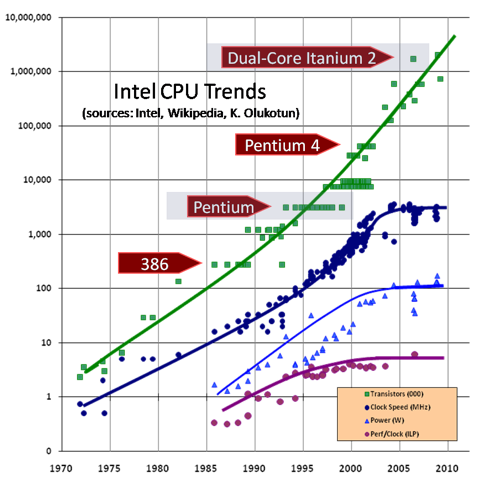
\includegraphics{images/cpu-chart.png}
		\caption{Processador Intel - velocidade de clock por transistores}
		\label{fig:cpu_chart}
		\end{figure}
		
		
	
		

\newpage
\bibliographystyle{abstract}
\bibliography{referencias}
\end{document}
